% Horizon penetrating coordinates (vs. Schwarzschild coordinates)
% for a black hole spacetime, with excision
% Author: Jonah Miller
\documentclass[tikz,border=0pt]{standalone}
\usepackage{tikz}
\usetikzlibrary{arrows}
\usetikzlibrary{arrows.meta}
\usetikzlibrary{decorations.markings}
\usepackage{pgfplots}
\usepackage{amsmath}
\usetikzlibrary{decorations.pathreplacing}
\usepackage{scalefnt}

\usepackage[utf8]{inputenc}

\usepgfplotslibrary{fillbetween}
\usepackage{lmodern}

\pgfmathsetseed{3}

%\tikzset{>={Latex[length=3mm]}}

\tikzstyle{mybox} = [draw=black,
    rectangle, inner sep=10pt, inner ysep=10pt]
\tikzstyle{fancytitle} =[fill=blue!30, text=black]

\pgfplotsset{soldot/.style={color=blue,only marks,mark=*}} \pgfplotsset{holdot/.style={color=blue,fill=white,only marks,mark=*}}


\begin{document}
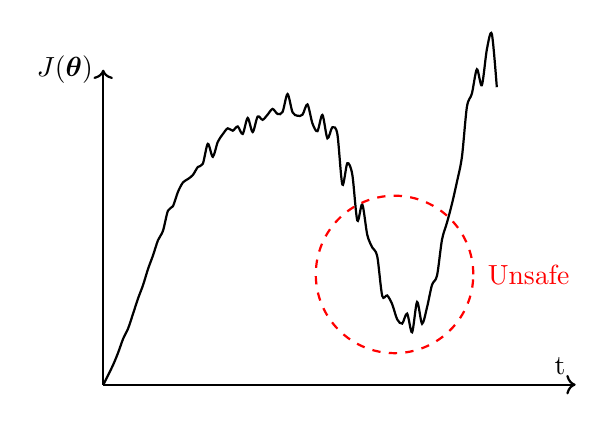
\begin{tikzpicture}

\draw[thick, ->] (0,0) -- (0,4) node[left]{$J(\boldsymbol{\theta})$};
\draw[thick, ->] (0,0) -- (6,0) node[above left]{t};

\draw[thick] plot [domain=0:5,smooth,samples=80] (\x,{0.9*(0.8*\x*sin(80*\x) + 0.3*\x*sin(160*\x)  + 2.1*\x  - 0.08*(\x)^2 + \x*0.1*rand - 3*e^(\x - 4)+0.05)});

\draw[red,thick,dashed] (4.7,1.4) arc (0:360:1) node[xshift=20]{Unsafe};


%\x*0.15*rand

\end{tikzpicture}
\end{document}